\section{Evaluation}
In this section we evaluate the implementation of our
approach across two case studies. 

These experiments aim at answering the following research questions:

1. RQ1: How do standard GCC optimization levels influence
on the resource consumption of running programs?
To answer this question, we apply standard optimization options to FFmpeg library. Then, we evaluate the memory footprint and execution time of running FFmpeg command lines and we
compare the results. The goal of this initial experiment is to
provide an understanding of the performance of
generated code by GCC.

2. RQ2: To what extent can the proposed diversity-based
exploration of optimization options impact the resource
consumption of generated programs?
In a second experiment, we assess our NS
approach for automatic optimization sequences generation by
comparing the results found when applying standard optimization sequences to new
results provided by our approach. In general, these experiments
show that our novelty-based approach produces optimization
sequences with higher performance and less resource consumption
than standard optimization levels in GCC. In this experiment, we focused as well on the tradeoff execution time/memory consumption.




\subsection{Case Study 1: FFmpeg}
In the first experiment, we set up our infrastructure for testing and monitoring the generated code. In this part, we compiled the FFmpeg library using standard GCC optimizations(O1, O2, O3, Ofast) and we studied the impact of these optimizations on memory consumption and execution time using our docker-based infrastructure.

\subsubsection{FFmpeg: Multimedia Encoding Library}
FFmpeg is a complete, cross-platform solution to record, convert and stream audio and video. It is a very fast video and audio converter. It processes a number of input files specified by the $-i$ option, and generate different output files according to the input plugin. FFmpeg allows different types of multimedia conversion and that depends on the input and output format (video, audio, subtitle, attachment, data).
Some command options have to be specified for each type of video or audio processing. In fact,
FFmpeg defines a set of option flags through command line to configure and generate the output
file (e.g. number of threads, size, bitrate, the video or audio codec). Video or audio processing with FFmpeg consumes lot of resources in term of memory usage. So, testing GCC on top of this library is very interesting. 
\subsubsection{Docker-based Infrastructure for monitoring FFmpeg containers}
\begin{figure}[h]
	\centering
	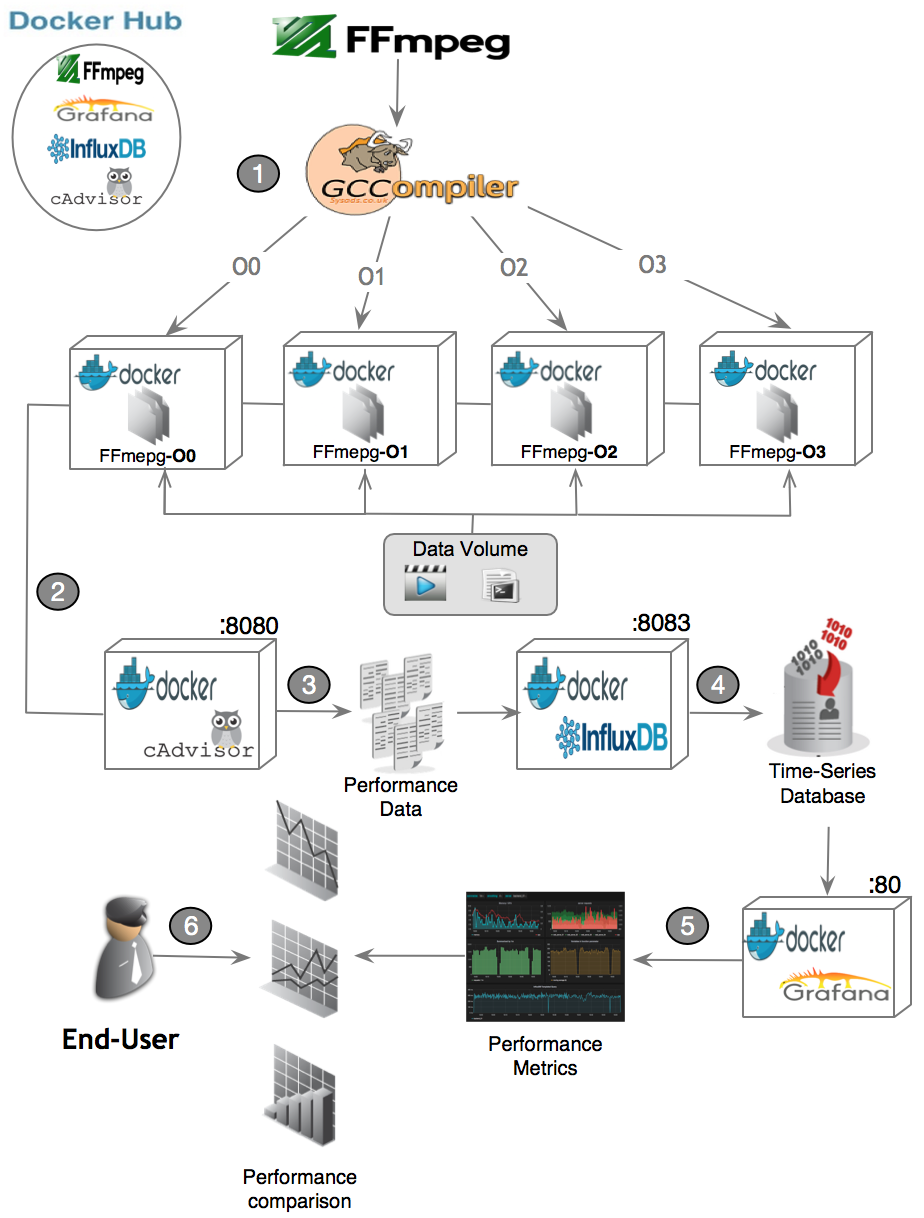
\includegraphics[scale=0.48]{Ressources/infra_ffmpeg.png}
	\caption{Overview of the different components involved in testing and monitoring of FFmpeg containers}
\end{figure}
\begin{figure*}
	
	\center
	
	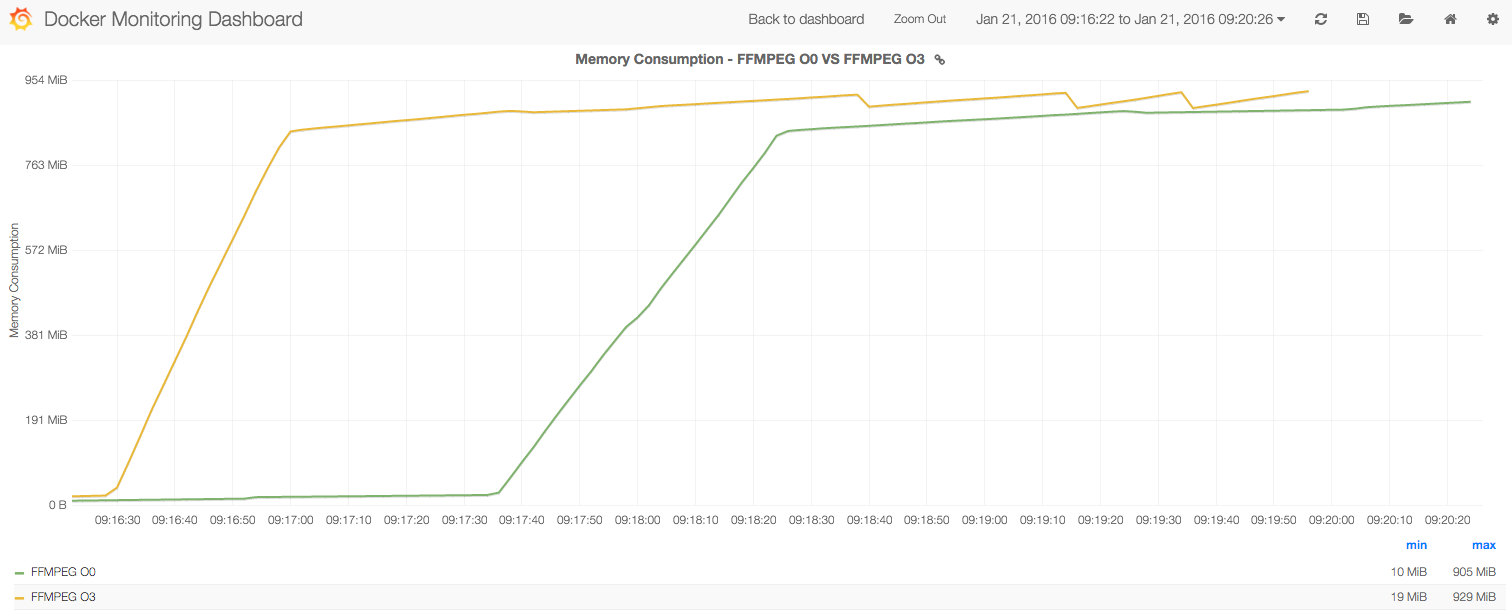
\includegraphics[width=15cm,height=7cm]{Ressources/infra_stats.png}
	\caption{Snapshot of runtime memory consumption profiles of FFmpeg containers compiled with O0 (no optimization) and O3 options}
	
	\label{AAA}
	
\end{figure*}
The goal of this experiment is to compile FFmpeg with standard GCC optimization options and run FFmpeg command examples on top of different versions in order to compare the memory usage profiles and execution time of different variants using our testing architecture. An overview of the different components involved in testing and monitoring of FFmpeg containers is shown in Figure 2. 
First, we compile FFmpeg library with different optimization options  (O0, O1, O2, O3 and Ofast) in order to produce 5 variants of FFmpeg. This is done within a Docker container with a Linux image. We configure
each container to install FFmpeg with a specific configuration and we uploaded all the FFmpeg images in Docker Hub\footnote{https://hub.docker.com/}.
Docker Hub is a cloud-based registry service for building and shipping application or
service containers. We are using it for building, saving and managing all our docker
images.
 Afterwards, we execute the same training FFmpeg examples within each FFmpeg instance container. We choose 15 FFmpeg command examples that cover multiple domains\footnote{http://goo.gl/11VLYM} like video conversion, sound extraction, encoding file for iPod or PSP, etc. This list of examples is saved in a script file that should be executed later within FFmpeg containers. The media files needed for encoding are saved in a shared repository. In docker environment, we call this repository the “Data Volume”. A data volume is a specially-designated directory within containers that share data with the host machine. Data is persistent and independent of container's life cycle. So, when we run FFmpeg containers we provide a shared volume with the host
machine (where the media files are located). As well, the list of FFmpeg commands to execute is mounted in this volume so that we can execute the same workload each time wr run a new container.

Before running the FFmepg workload on different containers, we run monitoring components (cAdvisor, InfluxDB and Grafana) to start gathering usage statistics.

Using Grafana, we are able to query database and define performance metrics. We use for this experiment to gather statistics about memory consumption and execution time of different containers. 

To obtain comparable and reproducible results, we used the same hardware across all experiments to run Docker: an AMD A10-7700K APU Radeon(TM) R7 Graphics processor with 4 CPU cores (2.0 GHz), running Linux with a 64 bit kernel and 16 GB of system memory.

\subsubsection{Experimental results}

The first part of this experiment is to compare the no-optimization container with the high-optimization one in order to study the impact of optimizations on resource consumption. Figure 3 shows runtime statistics for two running FFmpeg containers O0 and O3 with the same input workload. This chart presents the memory usage profile of two components (FFmpeg O0 and O3) started in the same time and running in parallel. Visually, we can see that the execution of O3 (yellow) is faster than O0 (green) by around 20s. However, we can see that memory usage remains higher than O0 from the beginning to the end of running the FFmpeg examples. 

To better understand resource usage of optimized containers, we run the same experiment for all FFmpeg containers and we collected the same metrics. Figure 4 presents a comparison of average memory usage and execution time of FFmpeg containers compiled with all standard GCC optimization options. We remark that the memory usage is increasing as soon as we apply more aggressive optimization.

This results explain that optimizing for execution time (for the case of FFmpeg) is not always efficient regarding memory usage and unfortunately, optimizations may influence negatively on system resources. 
\begin{figure}[h]
	\centering
	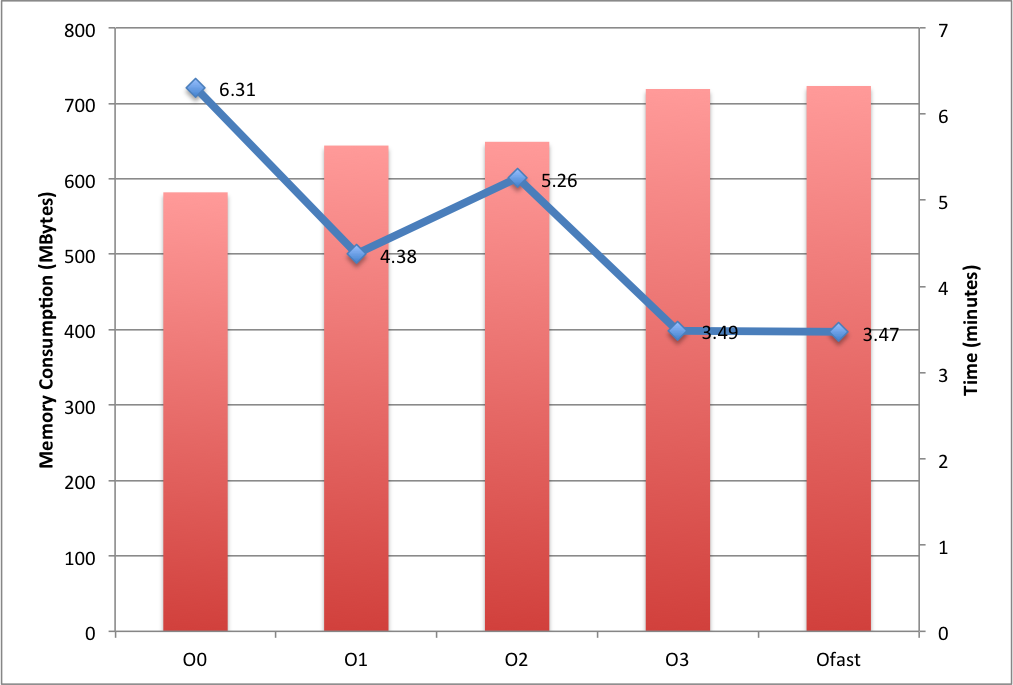
\includegraphics[scale=0.5]{Ressources/infra_ffmpeg_plot1.png}
	\caption{Comparison of average memory consumption and execution time of running workload in FFmpeg containers compiled with standard GCC optimization options}
\end{figure}


\subsection{Case Study 2: Novelty-based exploration of optimization sequences}
For the second experiment, we present a set of experiments to evaluate the performance optimized programs across target benchmarks. The goal of this section
is to show that our approach for exploring the search space of optimizations is able to generate efficient sequences of optimization options in term of performance and
resource consumption. We define an efficient sequence as a
set of optimization options that lead to use less resource consumption than GCC default optimizations.
\subsubsection{Approach}
\begin{figure}[h]
	\centering
	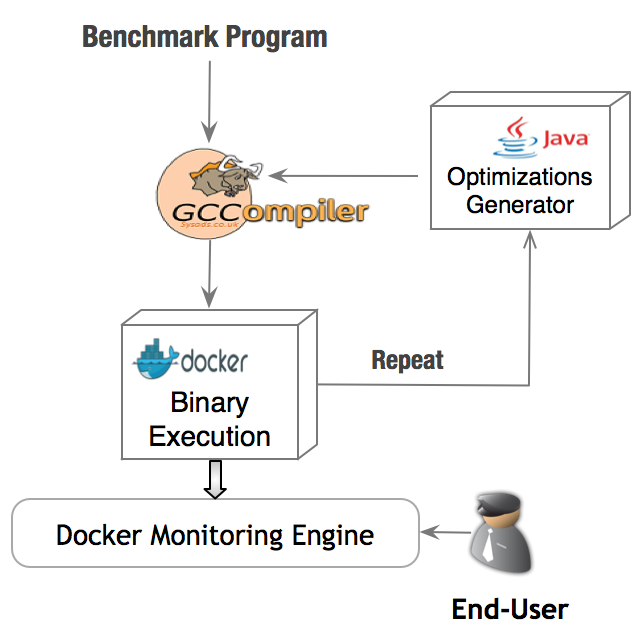
\includegraphics[scale=0.50]{Ressources/infra_novelty.png}
	\caption{Overall process of optimization space exploration and monitoring}
\end{figure}
We want to keep the same architecture settings as first case study for this experiment. However, in this example, we provide a more generalized approach for automatic testing of code generators using system containers. So, starting from a list of  optimizations defined by the used, an input program and a specific target compiler, we will be able to execute and monitor optimized code. Figure 5 shows more details about this process. First, our novelty-based test sequences generator will generate a huge amount of diverse optimizations. We compile an input program with these generated sequences using our GCC compiler. Then, program execution is done sequentially within isolated docker containers (docker image with GCC version 4.8.4 installed above). We keep the same monitoring chain to gather resource usage of running containers. This process is repeated until the end of generated sequences. Finally, end users (testers) can access to resource consumption statistics through InfluxDB or Grafana Web UI to compare the impact of optimizations on resource consumption. In this example too, we choose to focus on studying the trade-off memory usage/execution time. 
\subsubsection{Benchmark programs}
To explore the impact of compiler optimizations a set of test input programs are needed. We run experiments on commonly used benchmarks named Collective Benchmark (cBench)[ref]. It is a collection of open-source sequential programs in C targeting specific areas of the embedded market. It comes with multiple datasets assembled by the community to enable realistic benchmarking and research on program and architecture optimization. cBench contains more than 20 C programs. The following table describes programs that we have selected from this benchmark to evaluate our approach.
\begin{table}[h]
	\begin{center}
		\begin{tabular}{|c|c|p{4cm}|}
			\hline
			\textbf{Program} & \textbf{Source lines} & \textbf{Description}\\
			\hline
			automative\_susan\_s & 1376 & Image recognition package\\
			\hline
			bzip2e & 5125 & Compress any any file
			source code \\
			\hline
			bzip2d & 5125 & Decompress zipped files \\
			\hline
			office\_rsynth & 4111 & Text to speech program produced by integrating various pieces of code\\
			\hline
			consumer\_tiffmedian& 15870 & Apply the median cut algorithm to data in a TIFF file
			\\
			
			\hline
			 consumer\_tiffdither& 15399 & Convert a greyscale image to bilevel using dithering
			 \\
			\hline
			
		\end{tabular}
		
	\end{center}
	\caption {Description of selected benchmark programs}
\end{table}
\subsubsection{Novelty Parameters}
Our experiments use the classical NS algorithm, where we evolve a set of optimization sequences through generations.
NS is implemented as described in Section 3.
The first step in the process of selection is to evaluate each individual and compute its novelty score. Novelty is calculated for each organism by taking the mean of its 15 lowest dissimilar optimization sequences, by considering all sequences in the current population and in the archive. 

Then, to create next populations, an elite of the 10 most novel organisms is copied unchanged, after which the rest of the new population is created by tournament selection according to novelty. Standard genetic programming crossover and mutation operators are applied to these novel sequences in order to produce offspring individuals and fulfill the next population.

In the meanwhile, individuals that get a score higher than the threshold T they are automatically added to the archive as well. 

In fact, this threshold is dynamic. Every 1500 evaluations, it is checked how many individuals have been copied into the archive. If this number is below 3, the threshold is increased by multiplying it by 0.95, whereas if solutions added to archive are above 3, the threshold is decreased by multiplying it by 1.05. 

Moreover, as the size of the archive grows, the nearest-neighbor calculations that determine the novelty scores for individuals become more computationally demanding. So to avoid having low accuracy of novelty, we choose to bound the size of the archive. Hence, it follows a queue data structure (first-in first-out) which means that when a new solution gets added (enqueued), the oldest solution in the novelty archive will be discarded or dequeued. Thus, we ensure individuals diversity by removing old sequences that may no longer be reachable from the current population.

The parameters of the algorithm were tuned individually in preliminary experiments. For each parameter, a set of values was tested. The parameter values chosen are the mostly used in the literature[ref]. The value that yielded the highest performance scores was chosen. The resulting parameter values are listed in Table 4.
\begin{table}
	\begin{center}
		\caption{Parameters of the evolutionary algorithm}
		\begin{tabular}{ l l || l l }
			Parameter & Value & Parameter & Value \\	\hline
			Novelty nearest-k  & 15 &  Tournament size & 2\\ 
			Add archive prob. & 30 &  Mutation prob. & 0.1\\  
			Max archive size & 500 &  Crossover & 0.5  \\  
			Population size & 100 &  No generations &  100 \\  
			Individual length & 76 & Elitism & 10  \\ 
			Scaling archive prob. & 0.05 & Solutions added to archive & 3  \\ 
		\end{tabular}
	\end{center}
\end{table}

\subsubsection{Experimental results}
The goal of this experiment is to compare novelty-based generated sequences to standard GCC optimizations in term of memory consumption. Figure 6 shows this comparison across our set of benchmark programs. It presents the percentage of saved memory after applying standard and novelty optimizations comparing to O0 (no optimization applied).
For NS, we select the best sequence that reduces the memory consumption and we compare it to the memory footprint of O0, O1, O2, O3 and Ofast versions. The results show clearly that NS outperforms standard optimizations for all benchmark programs. Using NS, we were able to reach a maximum memory consumption reduction of almost 26\% for the case rsynth program against a maximum of 18\% reduction using Ofast option. As well, We remark that the impact of applying standard optimizations on memory consumption for each program differs from one program to another. we can see that using O1 for bzip2e and O2, O3 for tiffmedian can even increase by almost 13 \% the memory consumption (like the FFmpeg experiments). This agrees to the idea that standard optimizations does not produce always the same impact results on resource consumption and may be highly dependent on the benchmark and the source code they have been tested on. Our approach can clearly provide an alternative to catch most relevant optimization sequence regarding resource consumptions.


\begin{figure}[h]
	\centering
	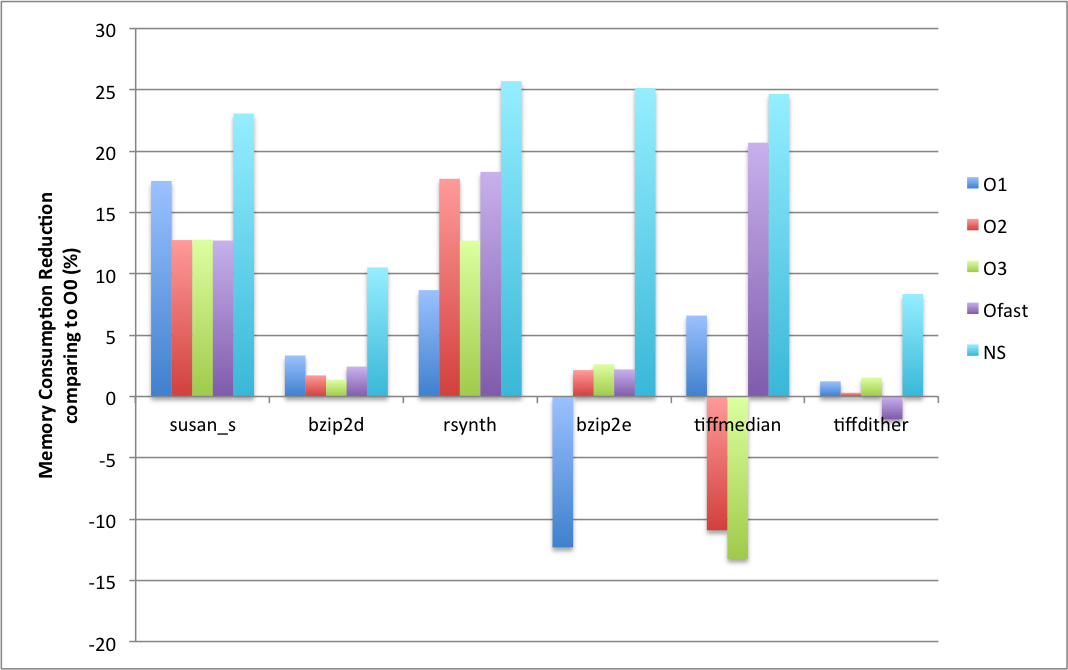
\includegraphics[scale=0.50]{Ressources/infra_novelty_stat3.png}
	\caption{Evaluating the amount of saved memory after applying standard optimization options comparing to new generated optimizations using NS}
\end{figure}
To study the correlation between execution time and memory consumption of running programs, we present in Figure 7 an evaluation of the speedup. We compared the speedup (according to O0) of the best optimization sequences by NS (gathered in Figure 6) and standard optimization options. 
\begin{figure}[h]
	\centering
	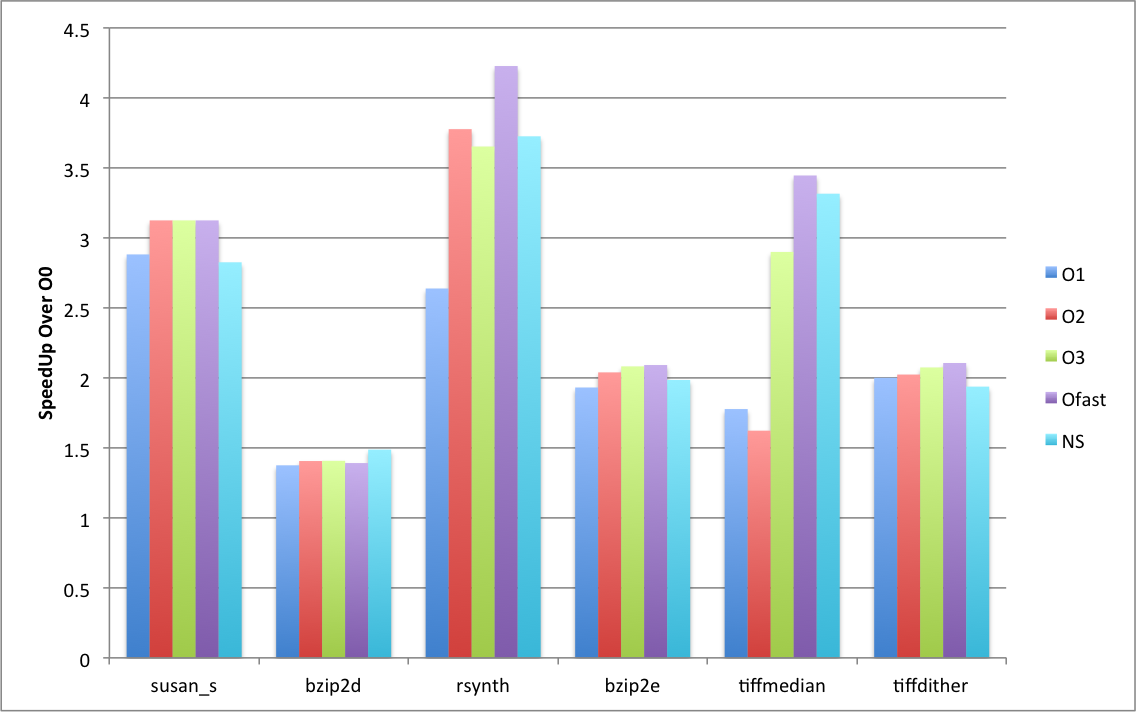
\includegraphics[scale=0.45]{Ressources/infra_novelty_stat2.png}
	\caption{Evaluating the speedup after applying standard optimization options comparing to new generated optimizations using NS}
\end{figure}
The first observation is that optimizations yields high level of speedup for all benchmarks (between 1.5 and 4.3).
The second observation we can make is that different optimizations do not differ too much in their
efficiency. We can distinguish that Ofast is slightly more efficient for all programs and NS sequence has almost the same speedup as Ofast. 

The results of this experiments shows that optimizing for resource usage using NS does not have an impact on the performance of program.

